\documentclass[border=10pt]{standalone}
\usepackage{tikz}
\usepackage{xcolor}
\usepackage{amsmath}
\usepackage{amssymb}

% Define colors
\definecolor{masterblue}{RGB}{52, 152, 219}
\definecolor{slavegreen}{RGB}{46, 204, 113}
\definecolor{networkorange}{RGB}{230, 126, 34}
\definecolor{taskpurple}{RGB}{155, 89, 182}
\definecolor{backgroundgray}{RGB}{236, 240, 241}

\begin{document}
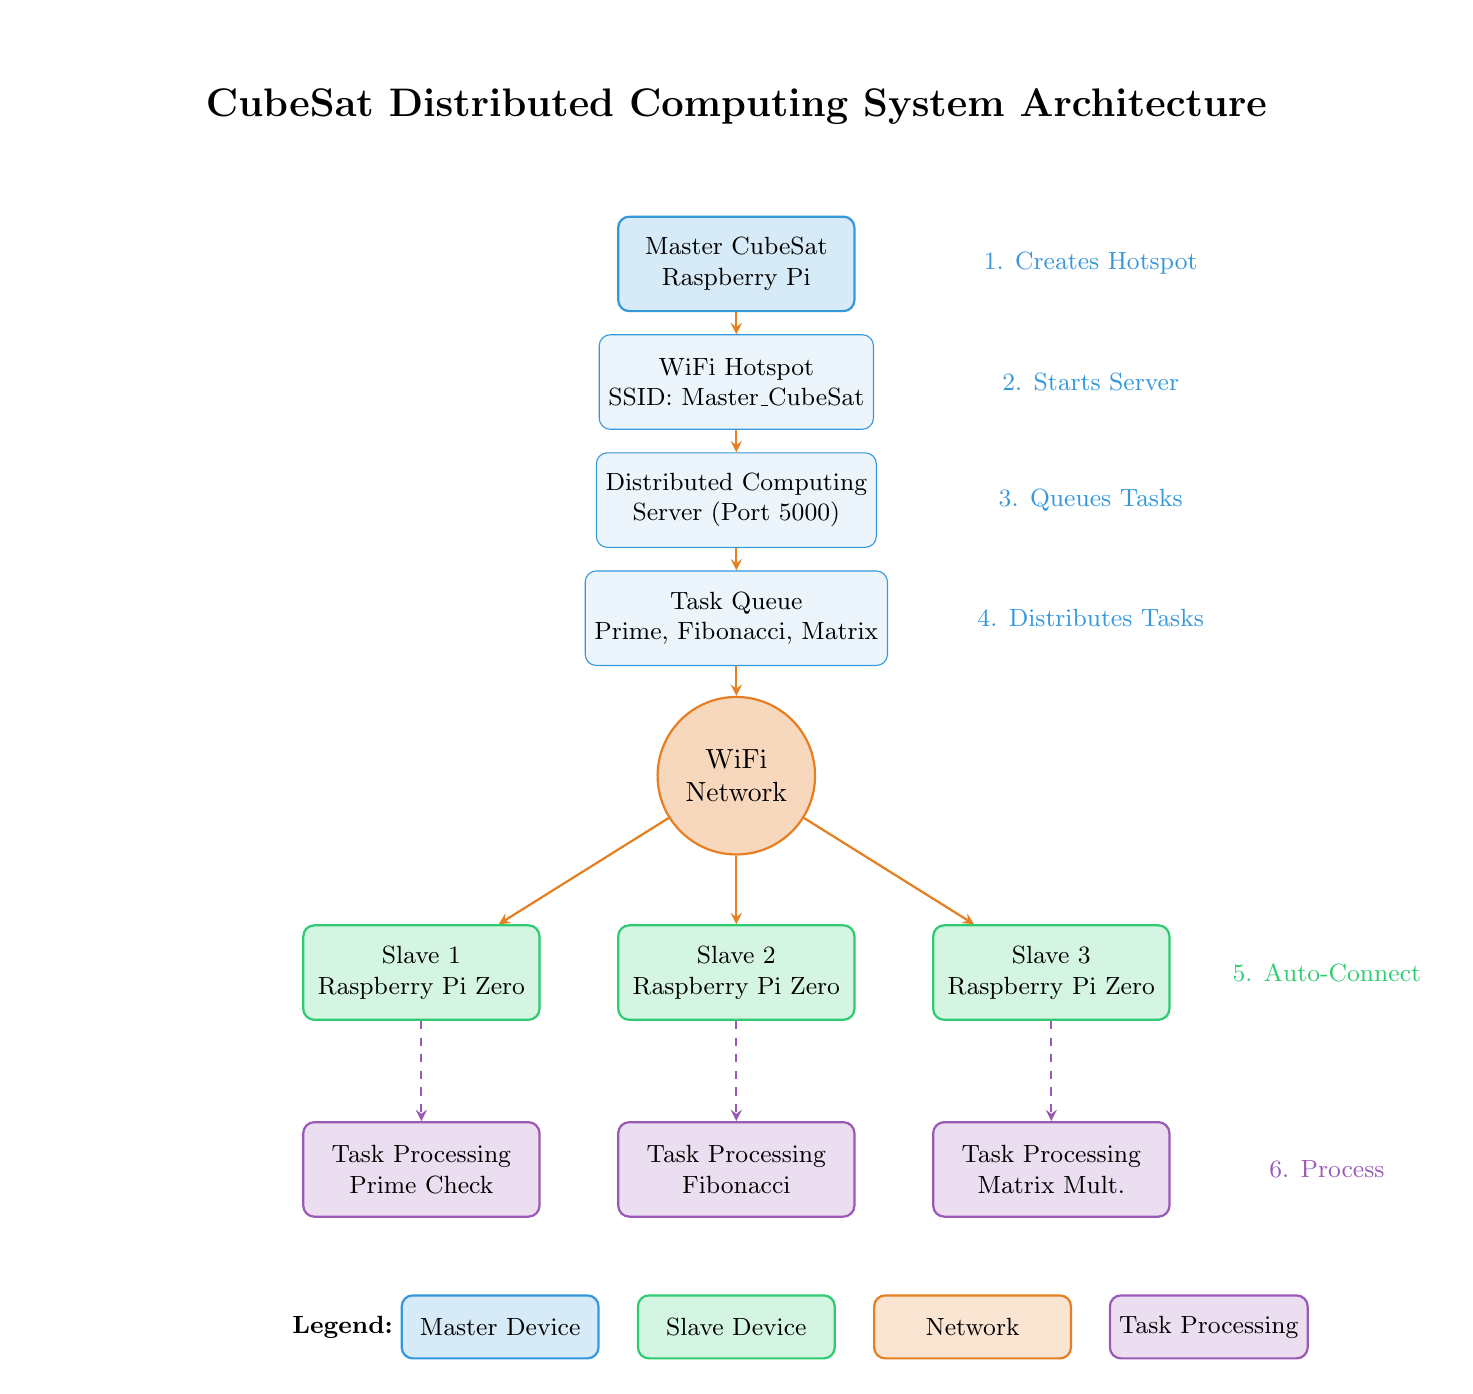
\begin{tikzpicture}[
    node distance=3cm,
    box/.style={rectangle, rounded corners, minimum width=3cm, minimum height=1.2cm, text centered, align=center, draw, font=\small},
    master/.style={box, fill=masterblue!20, draw=masterblue, thick},
    slave/.style={box, fill=slavegreen!20, draw=slavegreen, thick},
    network/.style={box, fill=networkorange!20, draw=networkorange, thick},
    task/.style={box, fill=taskpurple!20, draw=taskpurple, thick},
    arrow/.style={->, thick, >=stealth},
    wifi/.style={circle, minimum size=2cm, fill=networkorange!30, draw=networkorange, thick, align=center},
    dataflow/.style={->, thick, >=stealth, dashed, color=taskpurple},
    connection/.style={->, thick, >=stealth, color=networkorange},
    legendbox/.style={rectangle, rounded corners, minimum width=2.5cm, minimum height=0.8cm, text centered, draw, thick, font=\small}
]

% Background
\fill[white] (-3,-10) rectangle (15,7);

% Title
\node[font=\Large\bfseries] at (6,6) {CubeSat Distributed Computing System Architecture};

% Master CubeSat
\node[master] (master) at (6,4) {Master CubeSat\\ Raspberry Pi};
\node[box, fill=masterblue!10, draw=masterblue] (hotspot) at (6,2.5) {WiFi Hotspot\\ SSID: Master\_CubeSat};
\node[box, fill=masterblue!10, draw=masterblue] (server) at (6,1) {Distributed Computing\\ Server (Port 5000)};
\node[box, fill=masterblue!10, draw=masterblue] (taskqueue) at (6,-0.5) {Task Queue\\ Prime, Fibonacci, Matrix};

% WiFi Network
\node[wifi] (wifi) at (6,-2.5) {WiFi\\ Network};

% Slave Devices
\node[slave] (slave1) at (2,-5) {Slave 1\\ Raspberry Pi Zero};
\node[slave] (slave2) at (6,-5) {Slave 2\\ Raspberry Pi Zero};
\node[slave] (slave3) at (10,-5) {Slave 3\\ Raspberry Pi Zero};

% Task Processing
\node[task] (task1) at (2,-7.5) {Task Processing\\ Prime Check};
\node[task] (task2) at (6,-7.5) {Task Processing\\ Fibonacci};
\node[task] (task3) at (10,-7.5) {Task Processing\\ Matrix Mult.};

% Main connections (simplified to avoid overlaps)
\draw[connection] (master) -- (hotspot);
\draw[connection] (hotspot) -- (server);
\draw[connection] (server) -- (taskqueue);
\draw[connection] (taskqueue) -- (wifi);

% WiFi connections to slaves
\draw[connection] (wifi) -- (slave1);
\draw[connection] (wifi) -- (slave2);
\draw[connection] (wifi) -- (slave3);

% Task processing connections (one-way only)
\draw[dataflow] (slave1) -- (task1);
\draw[dataflow] (slave2) -- (task2);
\draw[dataflow] (slave3) -- (task3);

% Step labels (moved to avoid overlaps)
\node[font=\small, color=masterblue] at (10.5,4) {1. Creates Hotspot};
\node[font=\small, color=masterblue] at (10.5,2.5) {2. Starts Server};
\node[font=\small, color=masterblue] at (10.5,1) {3. Queues Tasks};
\node[font=\small, color=masterblue] at (10.5,-0.5) {4. Distributes Tasks};

\node[font=\small, color=slavegreen] at (13.5,-5) {5. Auto-Connect};

\node[font=\small, color=taskpurple] at (13.5,-7.5) {6. Process};

% Legend (text inside colored boxes)
\node[font=\small\bfseries] at (1,-9.5) {Legend:};
\node[legendbox, fill=masterblue!20, draw=masterblue, text=black] at (3,-9.5) {Master Device};
\node[legendbox, fill=slavegreen!20, draw=slavegreen, text=black] at (6,-9.5) {Slave Device};
\node[legendbox, fill=networkorange!20, draw=networkorange, text=black] at (9,-9.5) {Network};
\node[legendbox, fill=taskpurple!20, draw=taskpurple, text=black] at (12,-9.5) {Task Processing};

\end{tikzpicture}
\end{document}